% =============================
% VERSCHLÜSSELUNG DATEN
% =============================

\refstepcounter{chapter}
\chapter*{\thechapter. Datenverschlüsselung}
\addcontentsline{toc}{chapter}{\thechapter.\space Datenverschlüsselung}
Dieses Kapitel erläutert die Grundlagen und die Bedeutung moderner kryptografischer Verschlüsselungsverfahren,
die für die Sicherheit der heutigen digitalen Infrastruktur von zentraler Bedeutung sind. 
Zunächst wird die Funktionsweise von symmetrischen und asymmetrischen Verschlüsselungsverfahren beschrieben sowie die Funktionsweise der RSA-Verschlüsselung erklärt und deren Anwendungsgebiete aufgezeigt.
Anschliessend werden Methoden der Entschlüsselung erläutert, insbesondere der Brute-Force-Angriff. 
Des Weiteren wird der Shor-Algorithmus und dessen Zusammenhang mit dem Quantencomputer erklärt. Abschliessend wird die aktuelle Sicherheitslage heutiger Verschlüsselungsverfahren beurteilt und die Problematik der langfristigen Datensicherheit aufgezeigt.

\section{Funktionsweise moderner Verschlüsselung}
\subsection{Symmetrische Verschlüsselung}
Die symmetrische Verschlüsselung ist ein Kryptografieverfahren, bei dem derselbe geheime Schlüssel sowohl zum Verschlüsseln als auch zum Entschlüsseln von Daten verwendet wird. 
Auf dem Weg vom Sender zum Empfänger muss dieser Schlüssel sicher übertragen werden (siehe Abbildung \ref{fig:verschluesselung-symmetrisch}).
\begin{figure}[ht]
    \centering
    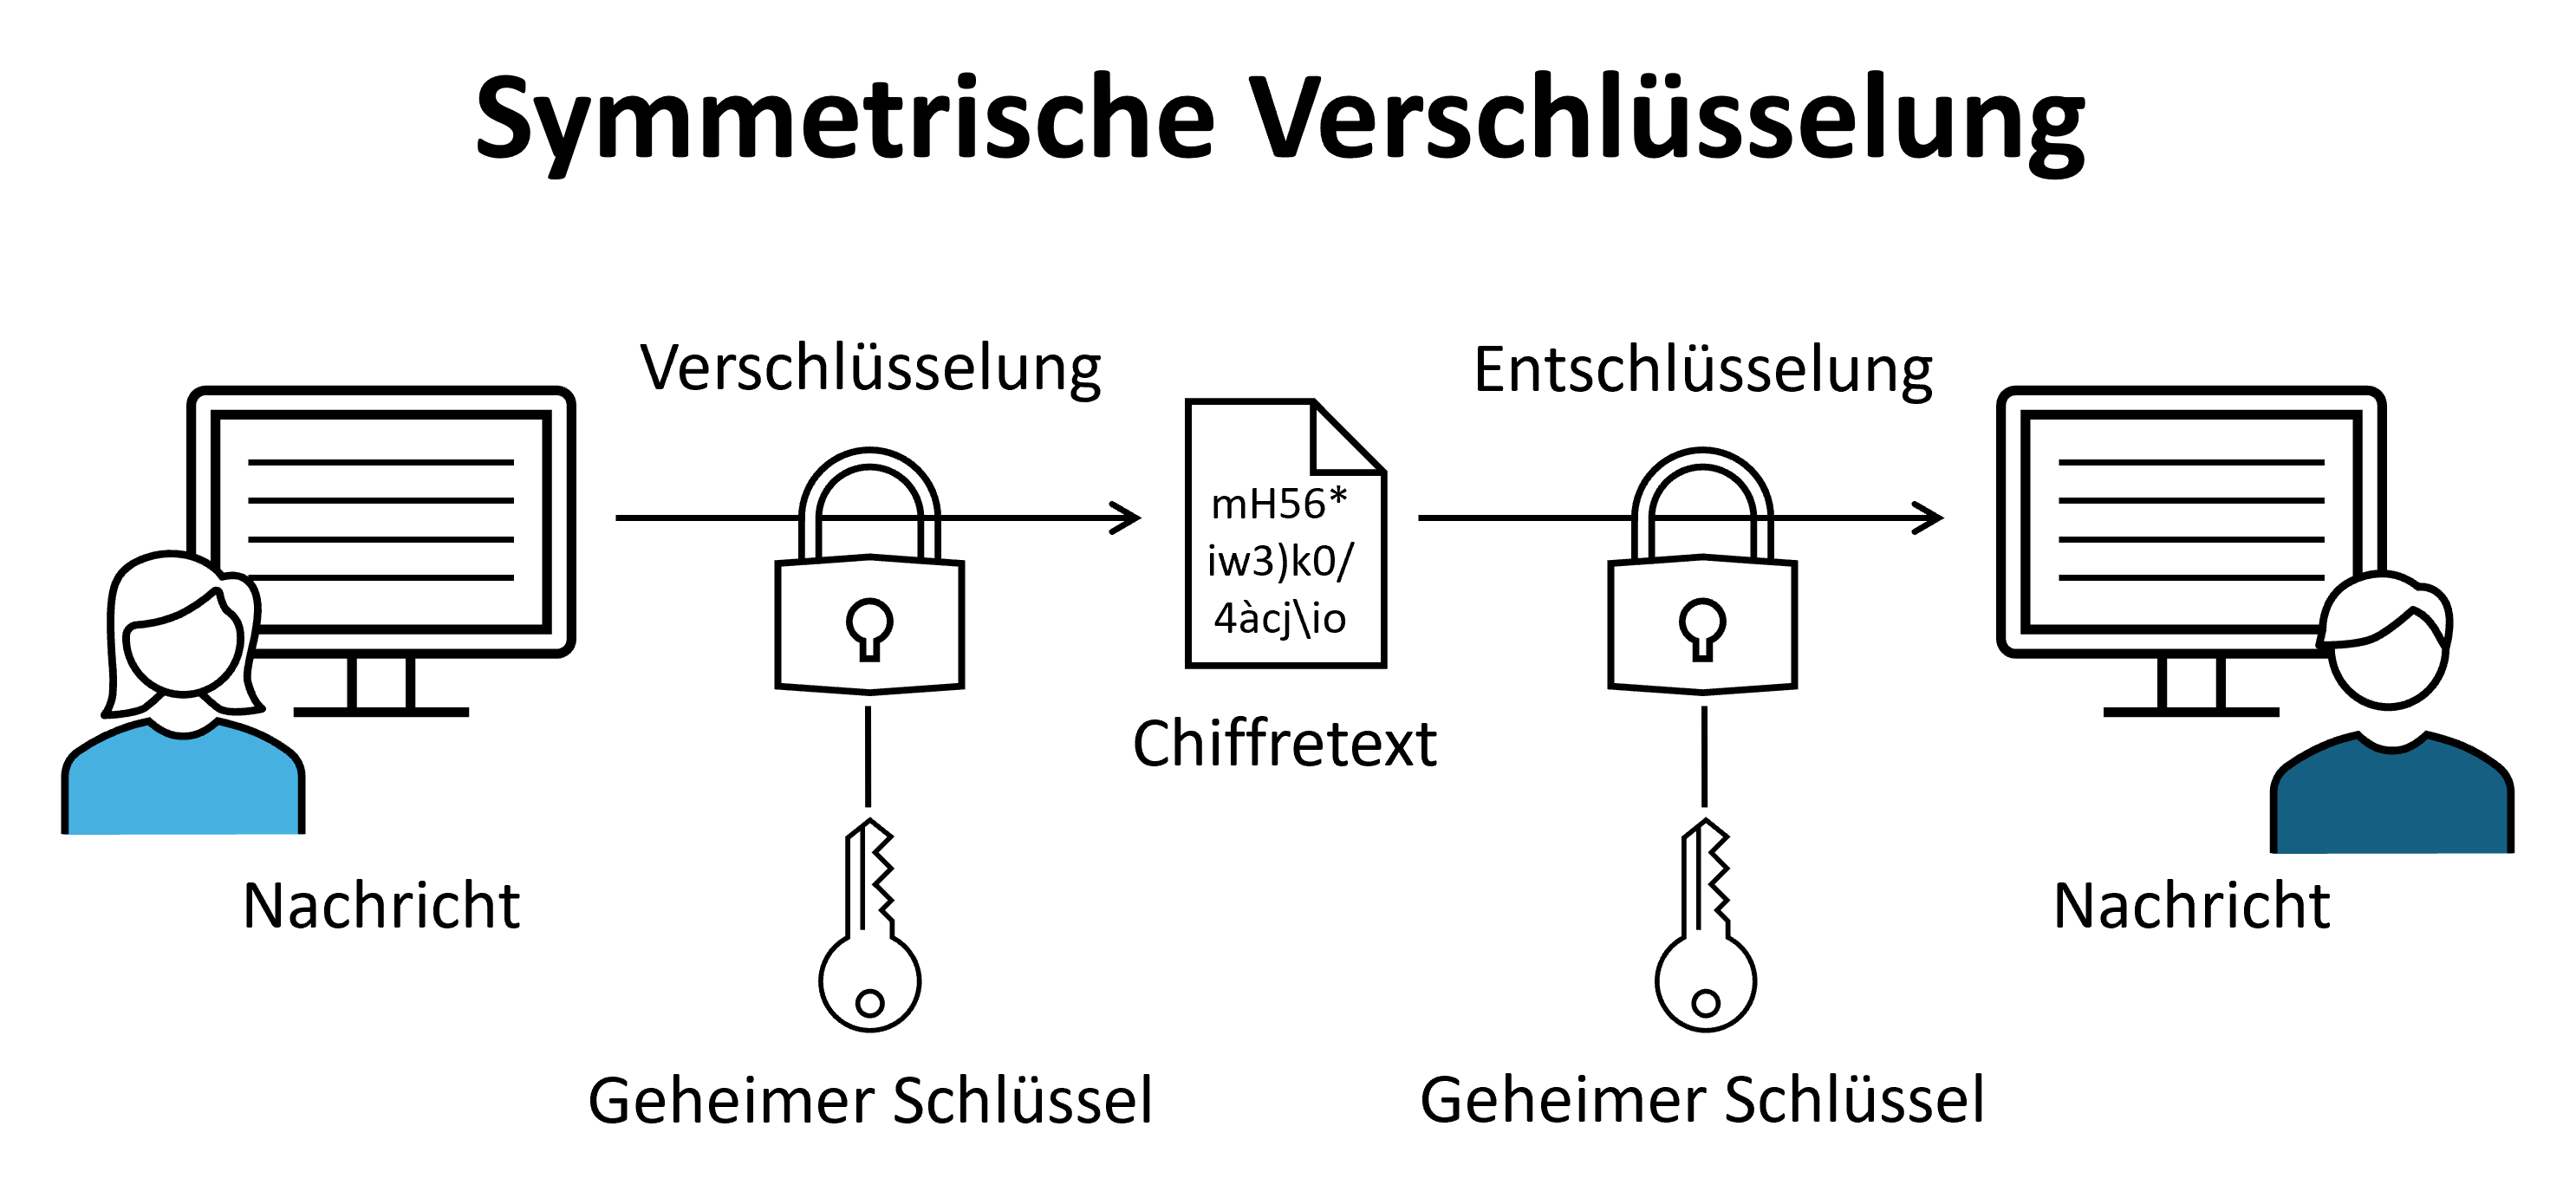
\includegraphics[height=0.25\linewidth]{images/Symmetrische_Verschluesselung.png}
    \caption{Funktionsweise der symmetrischen Verschlüsselung}
    \label{fig:verschluesselung-symmetrisch}
\end{figure}
Sobald dieser Schlüssel in die Hände eines Angreifers gelangt, sind alle Daten, die mit diesem Schlüssel geschützt sind, für den Angreifer lesbar \cite{nist800175b}. 
Ein historisches Beispiel der symmetrischen Verschlüsselung war die Enigma-Maschine im Zweiten Weltkrieg, welche zur Übertragung von militärischen Nachrichten und Informationen verwendet wurde. 
Genau wie bei einer symmetrischen Verschlüsselung besass diese Maschine einen Schlüssel, mit dem man diese Nachrichten entschlüsseln konnte.
Als die Engländer die Enigma-Maschine knackten, konnten sie alle Nachrichten entschlüsseln und auslesen, welche das deutsche Militär sendete. 
Daran zeigt sich das grundlegende Problem der symmetrischen Verschlüsselung:
Durch das einmalige Erhalten des Schlüssels, ist es ein Leichtes die Verschlüsselung auszulesen \cite{singh1999codebook}.


\subsection{Asymmetrische Verschlüsselung}
Asymmetrische Verschlüsselung wird auch Public-Key-Kryptografie genannt und verwendet ein Schlüsselpaar aus einem öffentlichen und einem privaten Schlüssel.
Asymmetrische Verschlüsselungsverfahren werden insbesondere eingesetzt, um einen sicheren Schlüsselaustausch in einem unsicheren Netzwerk zu ermöglichen.
Zusätzlich kann durch die asymmetrische Verschlüsselung eine digitale Signatur erstellt werden, wodurch die Authentizität und Integrität einer Nachricht überprüft werden kann \cite{nist800175b}.
Durch die mathematische Verknüpfung der beiden Schlüssel ist es möglich, dass eine Nachricht, die mit dem öffentlichen Schlüssel verschlüsselt wurde, nur mit dem privaten Schlüssel entschlüsselt werden kann.
Der öffentliche Schlüssel kann daher öffentlich verteilt werden, während der private Schlüssel geheim gehalten wird (siehe Abbildung \ref{fig:verschluesselung-asymmetrisch}). Die asymmetrische Verschlüsselungsverfahren werden insbesondere eingesetzt, um einen sicheren Schlüsselaustausch in einem unsicheren Netzwerk zu ermöglichen.
\begin{figure}[ht]
    \centering
    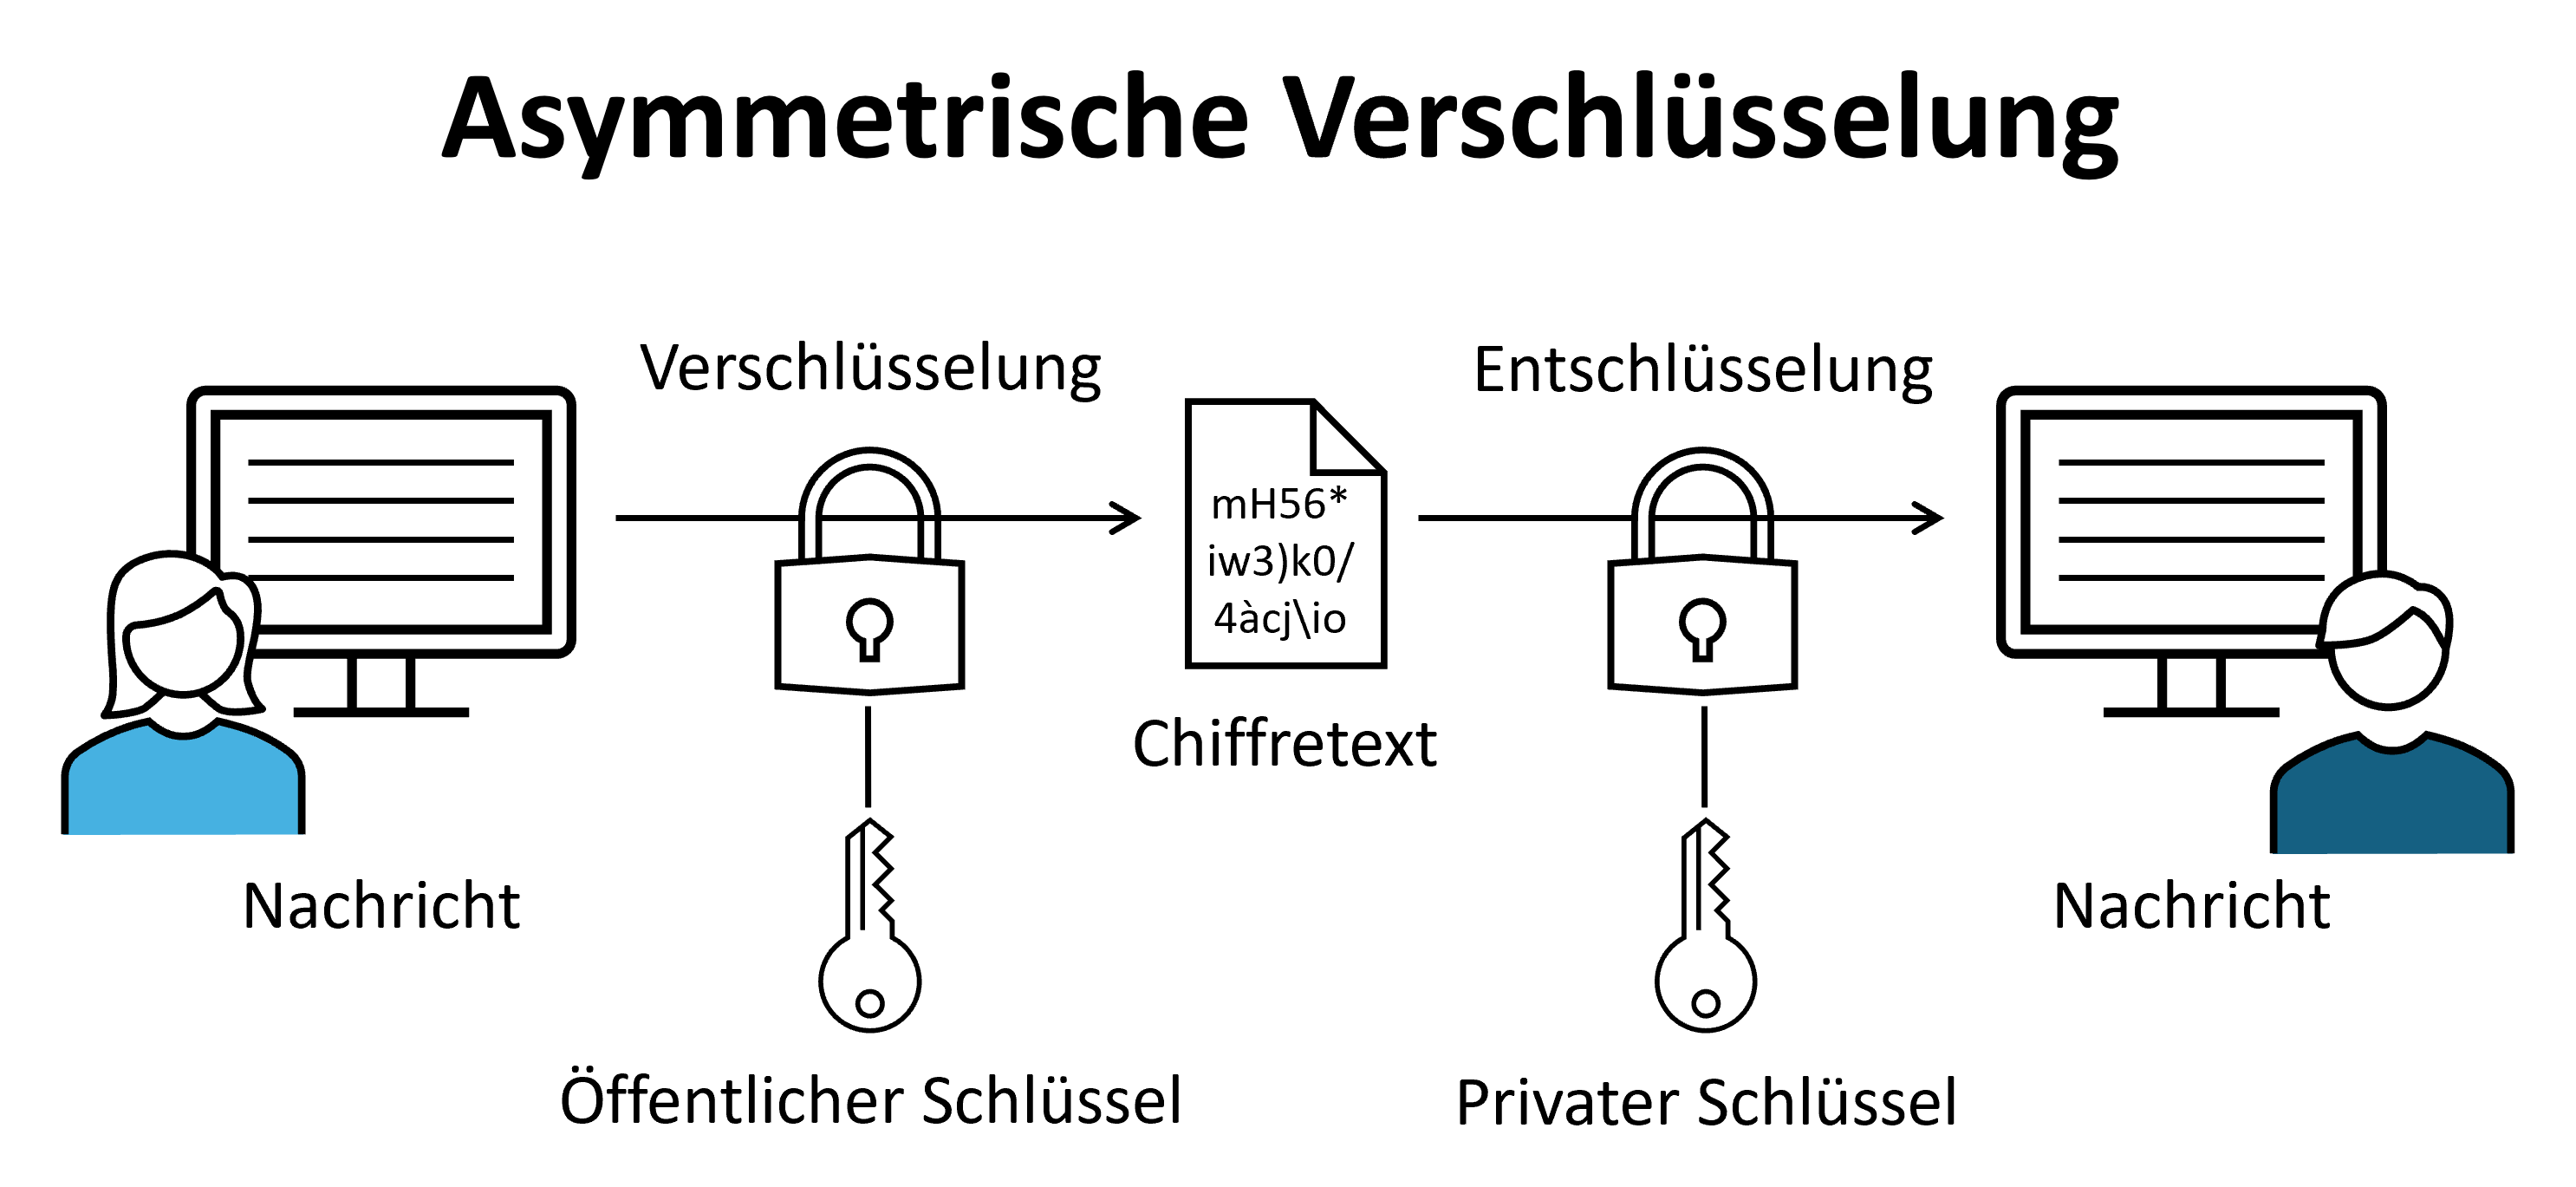
\includegraphics[height=0.25\linewidth]{images/Asymmetrische_Verschluesselung.png}
    \caption{Funktionsweise der asymmetrischen Verschlüsselung}
    \label{fig:verschluesselung-asymmetrisch}
\end{figure}
Die asymmetrische Verschlüsselung verursacht im Vergleich zur symmetrischen Verschlüsselung einen deutlich höheren Rechenaufwand.
Deshalb wird in der Praxis häufig nur die asymmetrische Verschlüsselung zur Übertragung von Sitzungsschlüsseln, also temporären, symmetrischen Schlüsseln, für eine Kommunikationssitzung verwendet.
Zusätzlich kann durch die asymmetrische Verschlüsselung eine digitale Signatur erstellt werden, wodurch die Authentizität und Integrität einer Nachricht überprüft werden kann \cite{nist800175b}.

\subsection{RSA-Verschlüsselungsverfahren}
Das Rivest-Shamir-Adleman-Verschlüsselungsverfahren (RSA) ist eines der bekanntesten und am weitesten verbreiteten asymmetrischen Verschlüsselungsverfahren. Es verwendet ein Schlüsselpaar aus einem öffentlichen und einem privaten Schlüssel.
Der öffentliche Schlüssel dient zur Verschlüsselung von Daten und Nachrichten, während der private Schlüssel zur Entschlüsselung verwendet wird.
Die Sicherheit des RSA-Verfahrens beruht auf der Schwierigkeit, extrem grosse Zahlen in ihre Primfaktoren zu zerlegen \cite{nist80056b}.
\\
Heute wird das RSA-Verfahren vor allem in digitalen Signaturen, Authentifizierungsmechanismen sowie beim sicheren Austausch symmetrischer 
Schlüssel eingesetzt. Aufgrund des hohen Rechenaufwands wird es nicht für die Verschlüsselung grosser Datenmengen verwendet.
Das National Institute of Standards and Technology (NIST) empfiehlt für RSA-Verfahren eine Mindestschlüssellänge von 2048 Bit, um eine ausreichende Sicherheit zu gewährleisten \cite{nist80056b}.
\pagebreak
\section{Methoden der Entschlüsselung}
Ein Algorithmus ist eine klare Schritt-für-Schritt-Anleitung, um ein Problem oder eine Aufgabe zu lösen, ähnlich wie ein Kochrezept.
Somit sagt er aus, welche nächsten Schritte zur Lösung eines Problems zu führen.
Da für die meisten Probleme verschiedene Algorithmen existieren, misst man diese typischerweise anhand des Ressourcenbedarfs, die sie benötigen, um das Problem zu lösen
z.B. der Laufzeit oder des Speicherbedarfs. 

\subsection{Brute-Force Angriff}
Ein Brute-Force-Angriff ist eine Methode in der Informatik und Kryptografie, 
bei dem eine grosse Menge an verschiedenen Passwörtern nahezu gleichzeitig 
ausprobiert werden, um das gesuchte Passwort oder den Verschlüsselungscode zu knacken (siehe Abbildung \ref{fig:brute_force_angriff}).
Es wird keinerlei Vorwissen oder ein Schlüssel benötigt, sondern eine riesige 
Menge unterschiedlicher Kombinationen ausprobiert, bis die richtige gefunden wurde \cite{owaspBruteForce}.
\begin{figure}[ht]
    \centering
    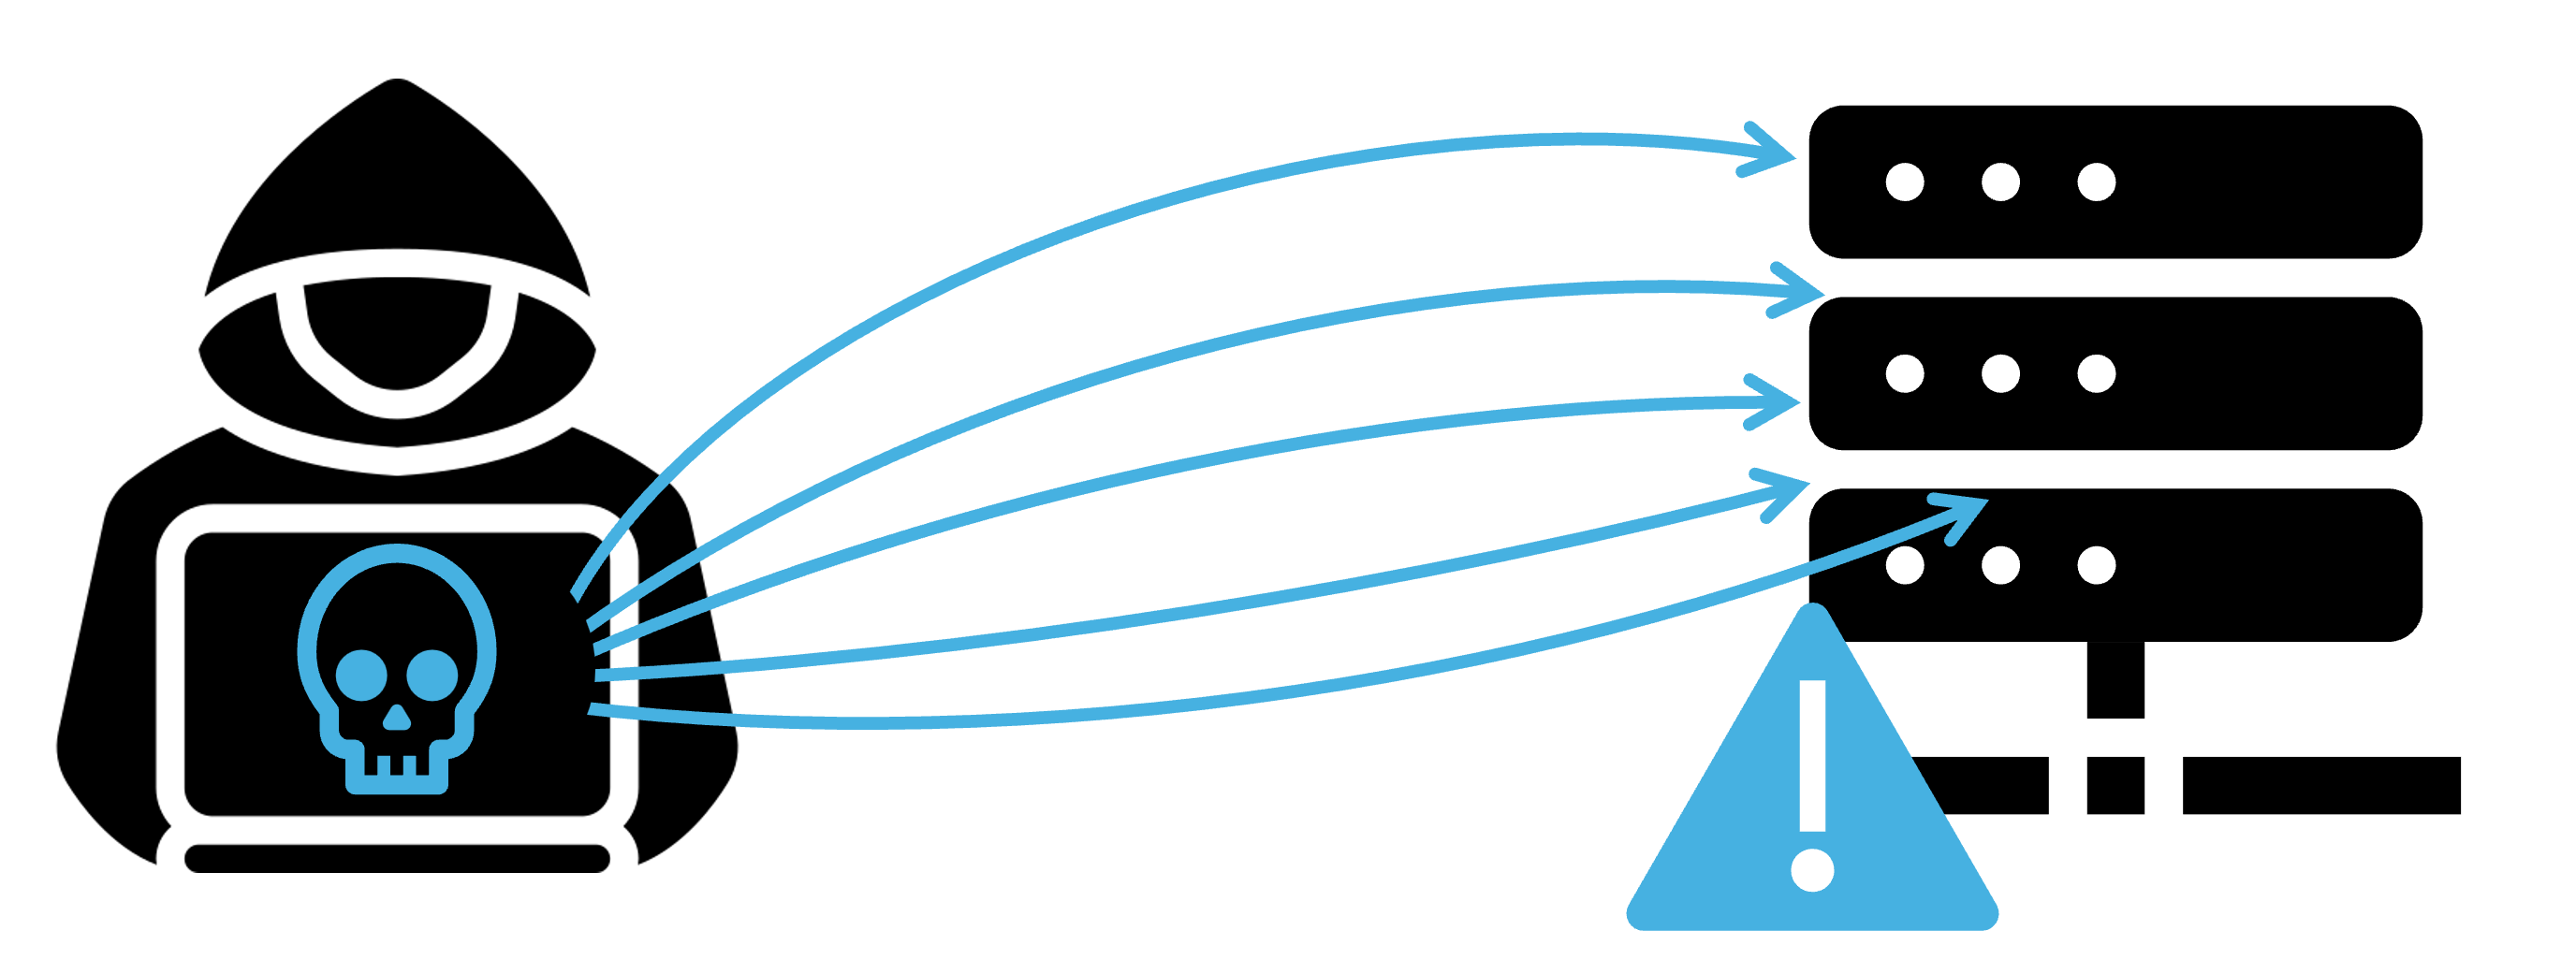
\includegraphics[height=0.25\linewidth]{images/Brute_Force_Attack.png}
    \caption{Funktionsweise des Brute-Force-Angriffs}
    \label{fig:brute_force_angriff}
\end{figure}
\\
Die Dauer eines sogenannten Brute-Force-Angriffs hängt von verschiedenen Faktoren ab, 
wie beispielsweise der Schlüssellänge, der Komplexität, des Zeichensatzes oder auch der 
Rechenleistung des Angreifers.
Kurze oder einfache Passwörter können dadurch innerhalb kurzer Zeit geknackt werden, 
während lange und komplexe Passwörter selbst mit der modernsten Hardware praktisch 
nicht mehr innerhalb einer realistischen Zeit entschlüsselbar sind.
Somit lohnt es nicht mehr, diese mit einem Brute-Force anzugreifen \cite{nist80063b}.
Um die Brute-Force-Angriffe zu verhindern, setzen heutige Systeme auf Schutzmechanismen 
wie eine Mindestlänge des Passworts, die Kombinationen aus Klein- und Grossbuchstaben, 
Zahlen und Zeichen, Sperrmechanismen nach Fehlversuchen sowie das 
\hyperlink{hashen-def}{Hashen} von Passwörtern \cite{nist80063b} \cite{menezes1996handbook}.
Der LinkedIn-Vorfall im Jahr 2012 zeigt, wie wichtig es ist, sich vor solchen Angriffen 
zu schützen und lange und komplexe Passwörter zu verwenden.
Hacker hatten damals 6,5 Millionen Passwörter von LinkedIn-Nutzern gehashed und veröffentlicht \cite{linkedinBreach}.
\\
Das folgende Beispiel zeigt den Schutzmechanismus gegen einen Brute-Force-Angriff auf:
Ein 8-stelliges Passwort aus Kleinbuchstaben hat $26^8 = 2,1*10^{11}$ mögliche Variationen.
Mit einer Rechenleistung von 1 Milliarde Versuchen pro Sekunde würde ein Brute-Force-Angriff 
etwa 208 Sekunden dauern.
Bei einem 12-stelligen Passwort aus Gross- und Kleinbuchstaben sowie Zahlen und 
Sonderzeichen (ca. $72^{12} = 1,94 * 10^{22}$ Variationen) würde derselbe Angriff etwa 
615'000 Jahre dauern \cite{wikipedia_bruteforce_passwords}.

\newpage
\subsection{Shor-Algorithmus}
\label{sec:Shor-Algorithmus}
\hypertarget{shor_algorithm}{}
Der Shor-Algorithmus wurde 1994 von Peter W. Shor entwickelt und gilt als einer der bekanntesten Quantenalgorithmen. 
Er löst zwei zentrale mathematische Probleme in \hyperlink{polynomialtime}{Polynomzeit}: die Zerlegung sehr grosser Zahlen in ihre Primfaktoren sowie das Berechnen des ganzzahligen Logarithmuses. 
Ein normaler Algorithmus benötigt für diese Probleme eine exponentielle Zeit, was sie für grosse Zahlen praktisch unlösbar macht \cite{mandrysch2016}.
Den Ablauf des Shor-Algorithmuses zeigt Abbildung \ref{fig:shor_algorithmus_sequence}.
\begin{figure}[ht]
    \centering
    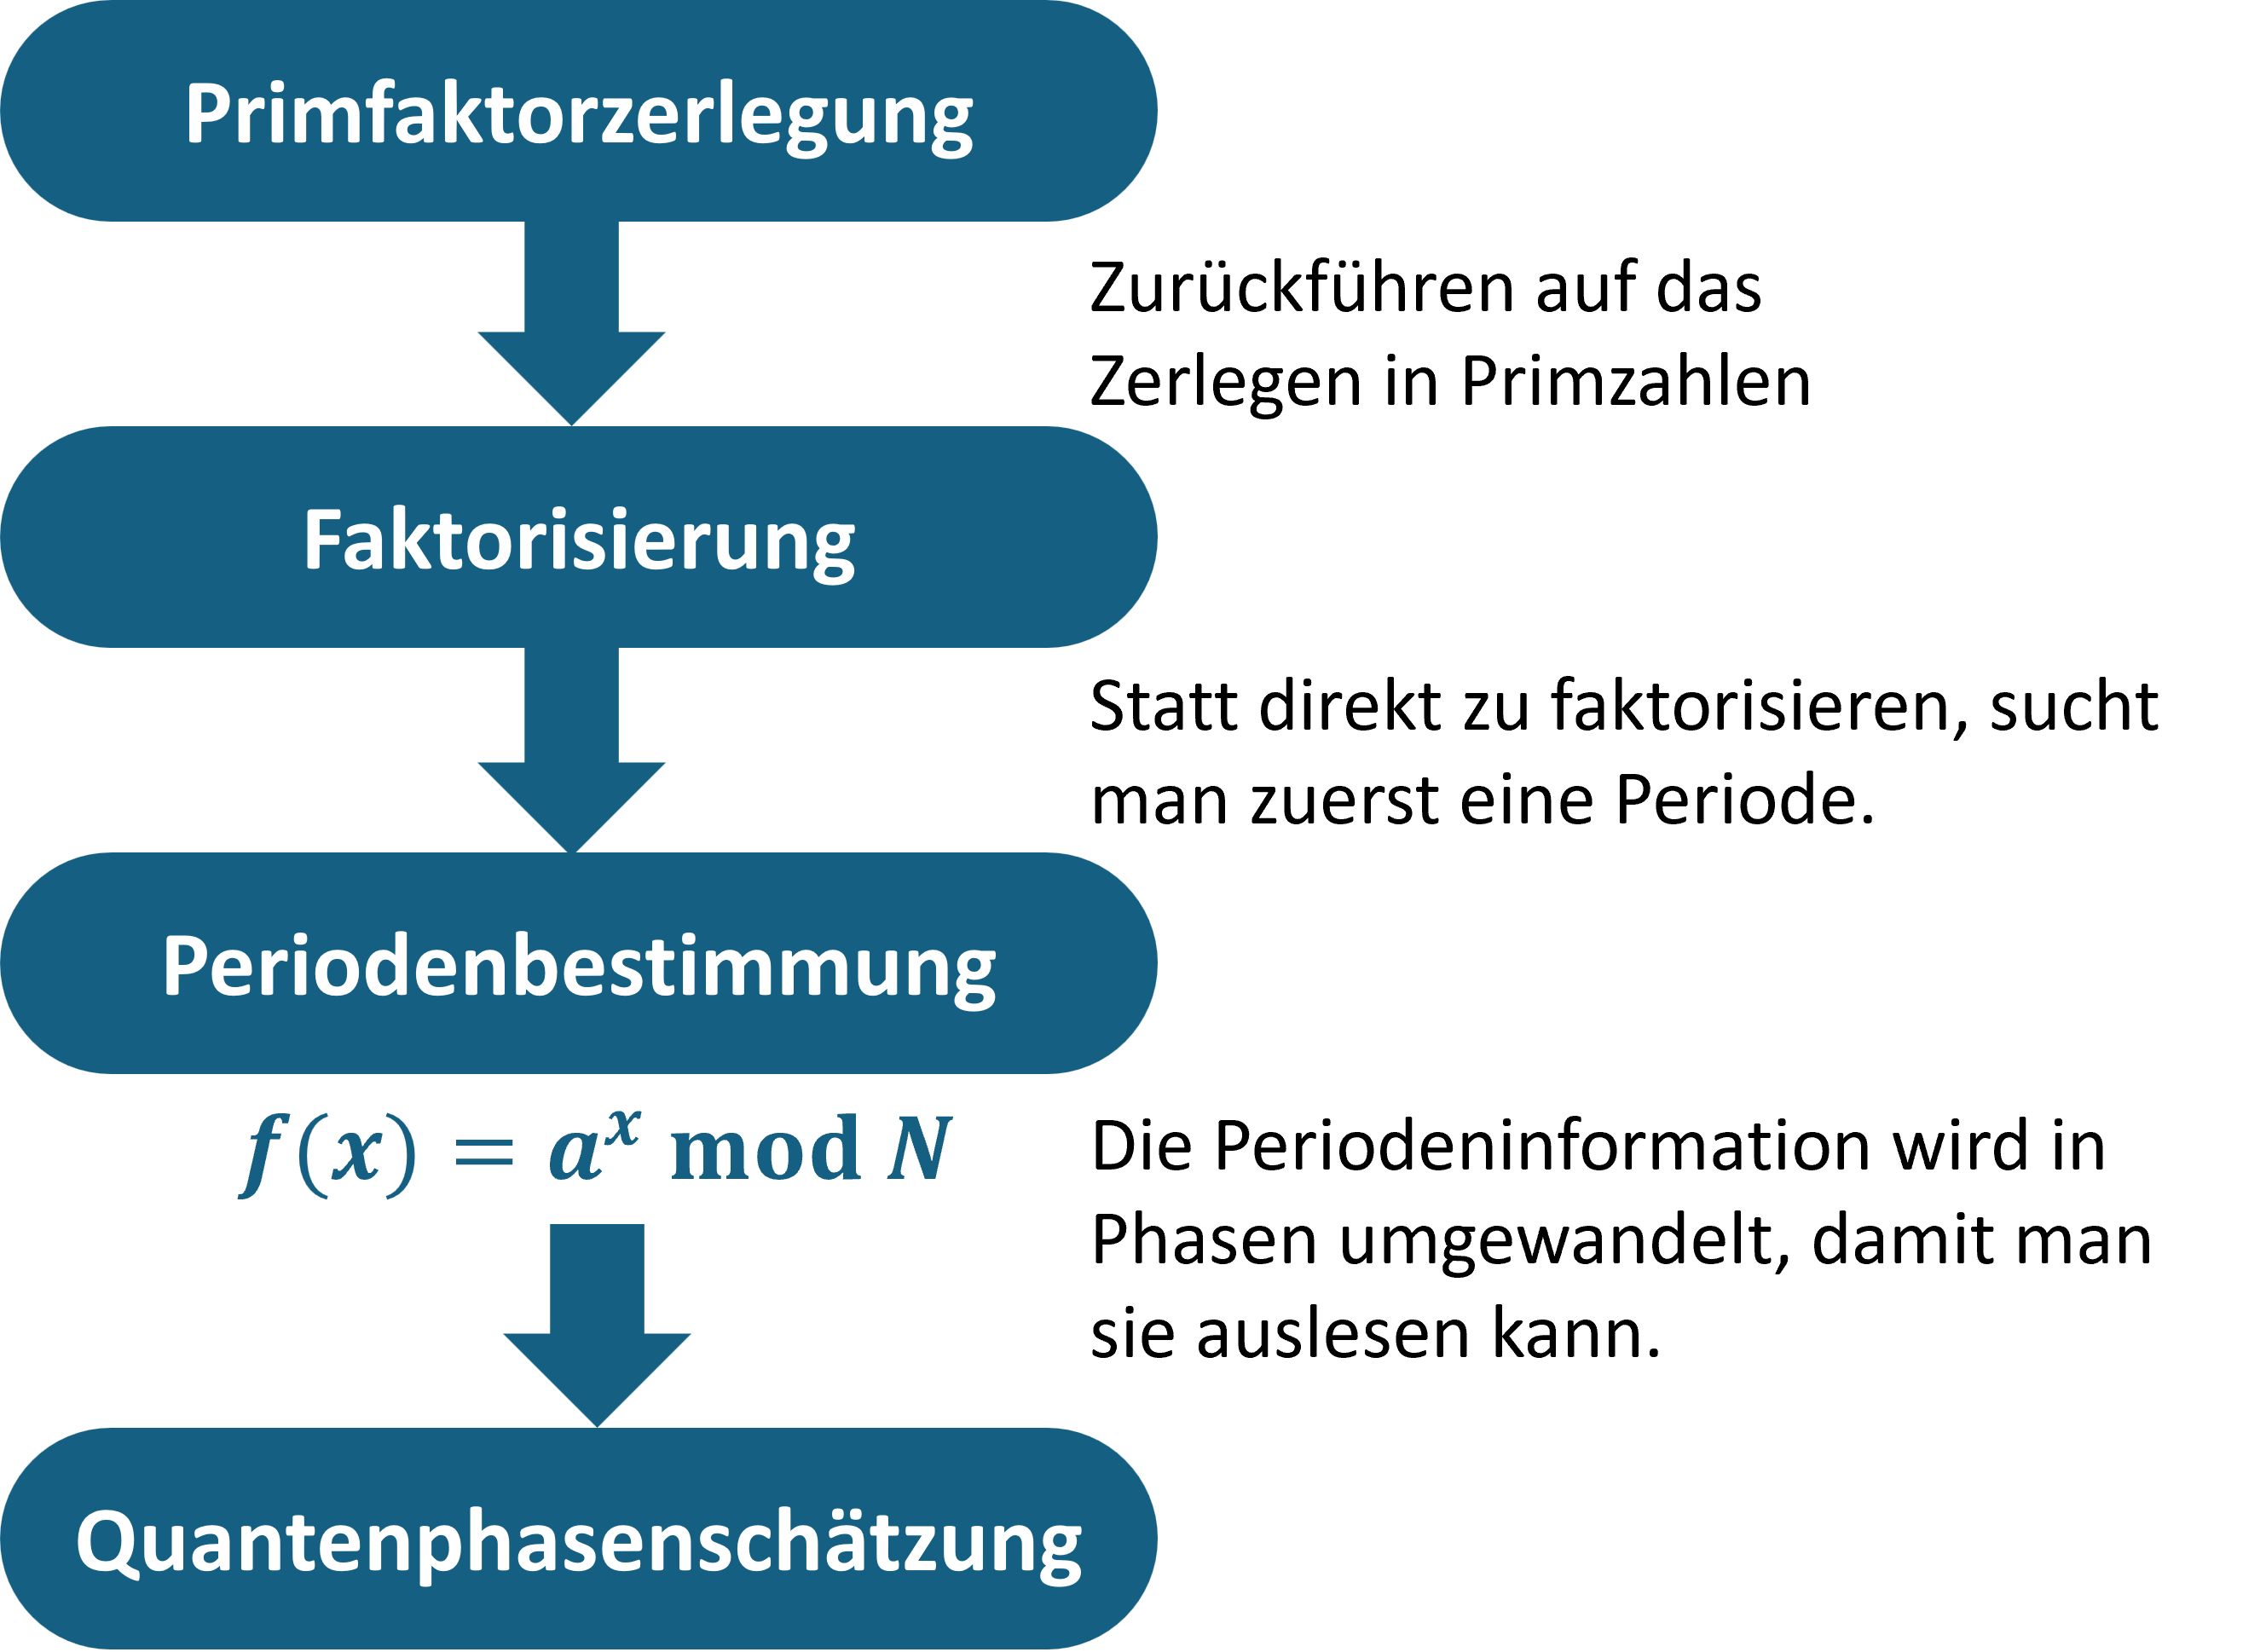
\includegraphics[height=0.38\linewidth]{images/Shor_Algorithm_Sequence.png}
    \caption{Funktionsweise des Shor-Algorithmus, (Quelle: \cite{mandrysch2016} - teilweise modifiziert).}
    \label{fig:shor_algorithmus_sequence}
\end{figure}
\\Der Shor-Algorithmus wird im Quantencomputer durch Quantengatter (siehe Kapitel 2.2) umgesetzt. 
Diese bilden die Bausteine, mit denen der Algorithmus physikalisch realisiert wird.
\\
Zu Beginn des Algorithmus werden Hadamard-Gatter auf mehrere Qubits angewendet. 
Sie erzeugen eine Superposition, sodass der Quantencomputer viele mögliche Rechenwege gleichzeitig verfolgen kann. 
Während ein klassischer Computer jeden Wert einzeln ausprobieren müsste, kann der Quantencomputer diese Berechnungen parallel durchführen.
\\
Anschliessend kommen kontrollierte Quantengatter wie CNOT- und kontrollierte Phasengatter zum Einsatz. 
Sie verschränken die Qubits miteinander, sodass ihre Zustände voneinander abhängen. 
In diesem Schritt wird die folgende Funktion ausgewertet:
\begin{equation*}
    f(x)=a^x \bmod N
\end{equation*}
Dabei werden Potenzen von $a$ berechnet und jeweils nur der Teilerrest (auch \hyperlink{modulo-def}{Modulo} genannt) von $\frac{a^{x}}{N}$ betrachtet. 
Die so entstehenden Werte wiederholen sich nach einer gewissen Anzahl Schritte, diese Wiederholung nennt man Periode.
Der Quantencomputer speichert diese Periodeninformation nicht als klassische Zahl, sondern repräsentiert sie in den relativen Phasen (Winkel \(\varphi\) der Bloch-Kugel) der Qubits. 
\\
Der wichtigste quantenmechanische Schritt ist anschliessend die Quanten-\hyperlink{fourier-transform-def}{Fourier-Transformation} (QFT). 
Sie besteht aus einer Abfolge von Hadamard-Gattern und kontrollierten Rotationsgattern \(R_k\), welche die Phasen der Qubits gezielt verändern. 
Dadurch wird die zuvor versteckte Periodeninformation so umgeformt, dass sie bei der anschliessenden Messung sichtbar wird. 
Zum Schluss korrigieren SWAP-Gatter die Reihenfolge der Qubits, da die QFT die Resultate in umgekehrter Bitreihenfolge liefert.
Kennt man die Periode, lassen sich daraus mit klassischen Rechenschritten die Primfaktoren der ursprünglichen Zahl bestimmen \cite{mandrysch2016}.
Abbildung \ref{fig:shor_algorithm_symbolic} zeigt eine vereinfachte Darstellung des Quantenschaltkreises für den Shor-Algorithmus.
\\
\begin{figure}[ht]
    \centering
    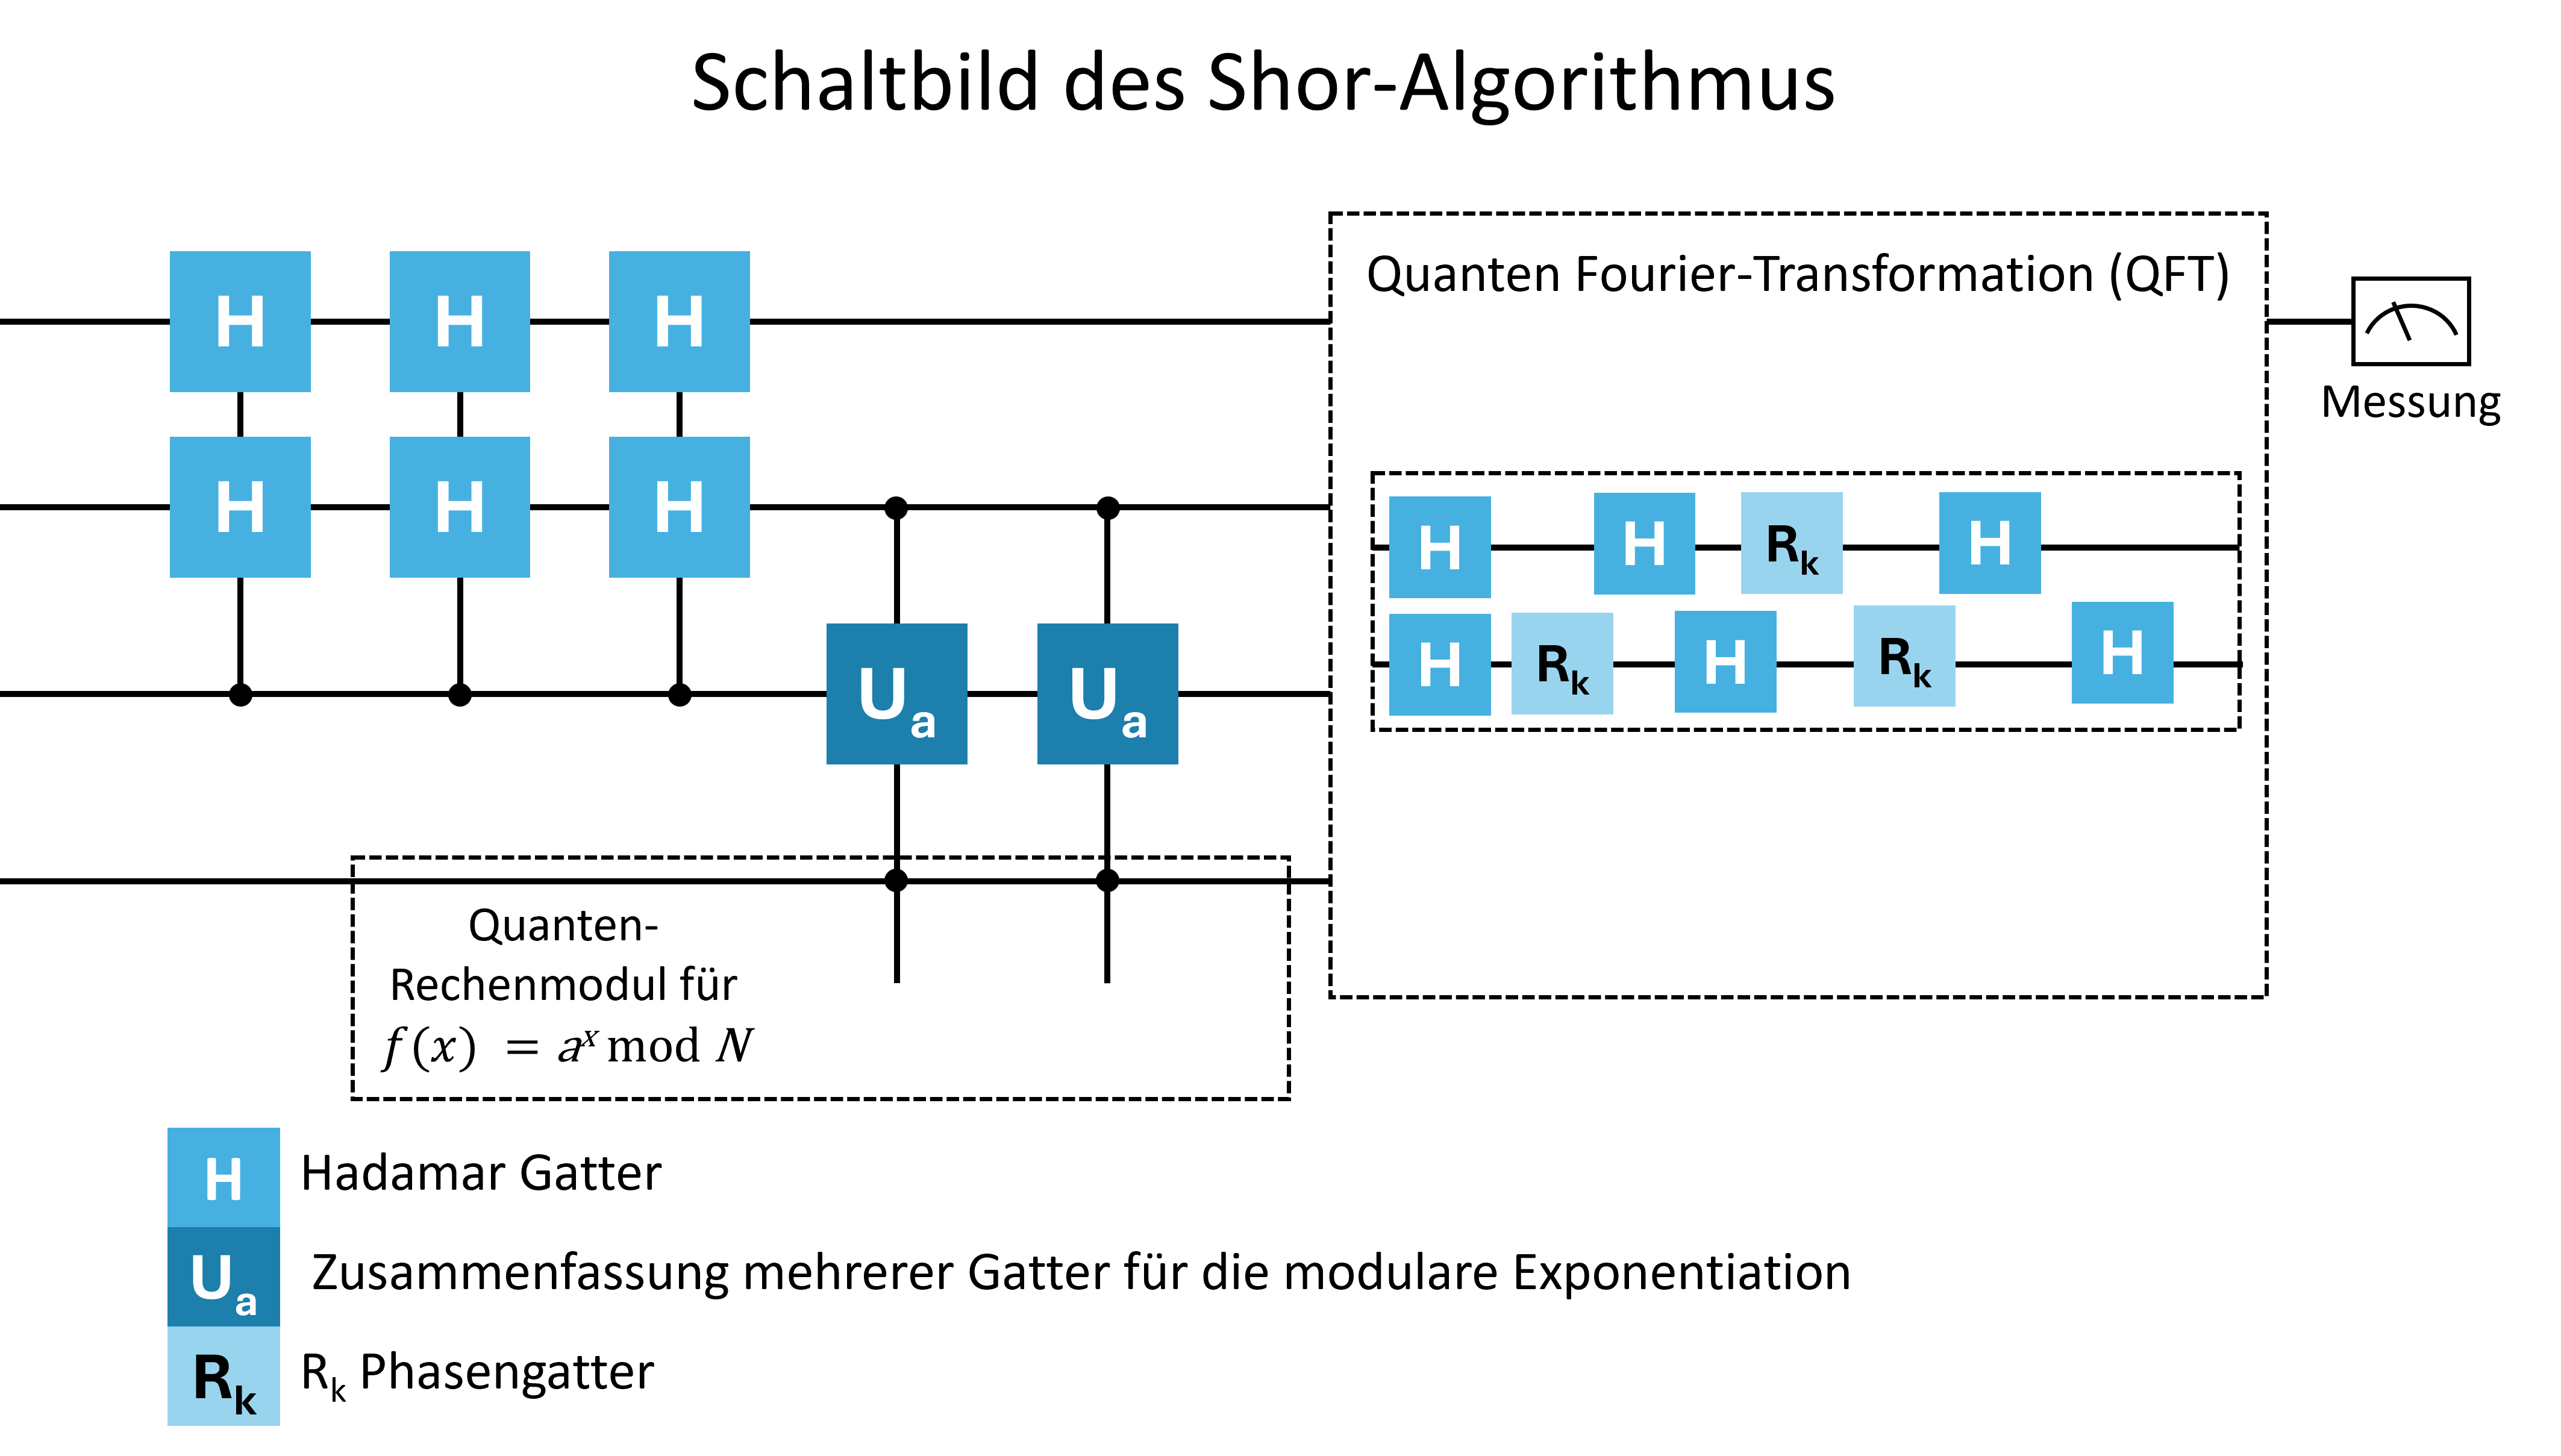
\includegraphics[width=0.75\linewidth]{images/Shor_Algorithm_quantum_circuit.png}
    \caption{Ablauf des Shor-Algorithmus (Quelle: \cite{bashiri2025quantencomputing} - teilweise modifiziert).}
    \label{fig:shor_algorithm_symbolic}
\end{figure}
\\[1em]
Wird beispielsweise der RSA-Algorithmus mit einer Schlüssellänge von 2048 Bit und einer Sicherheitsstufe von 112 Bit verwendet,
dann würde ein herkömmlicher Algorithmus mehrere Milliarden Jahre benötigen, um den zugehörigen privaten Schlüssel durch Primfaktorzerlegung zu berechnen.
Durch den Shor-Algorithmus könnte dieser Schlüssel mit einem ausreichend leistungsfähigen Quantencomputer innerhalb von Stunden bestimmt werden.
Konkret bedeutet das, dass ein klassischer Algorithmus ca. $5*10^{33}$ Rechenschritte benötigt, um den Schlüssel zu berechnen, während der Shor-Algorithmus lediglich 
$9*10^{9}$ Rechenschritte benötigen würde \cite{mandrysch2016}.
\\
Der aktuelle Rekord (Stand 2019) für die Faktorisierung mit dem Shor-Algorithmus liegt bei 65531, welche in die Primfaktoren 19 und 3449 zerlegt wurde \cite{fzJuelichShor}.
Dies ist weit davon entfernt, die Verschlüsselungstechnik zu revolutionieren.
Heutige Verschlüsselungsverfahren nutzen semiprime Zahlen (also Zahlen mit genau zwei Primfaktoren) mit mehreren hundert Stellen \cite{srfEinsteinQuantencomputer}. 
Dabei steigt der Bedarf an Qubits linear mit der Bitlänge der Zahl an, was die Faktorisierung grosser Zahlen (z.B. 2048 Bit) aktuell unmöglich macht \cite{fzJuelichShor}. 

\newpage
\section{Beurteilung der aktuellen Sicherheit}
Verschlüsselungsverfahren sind heute in nahezu allen digitalen Bereichen unverzichtbar.
Sie stellen sicher, dass digitale Informationen vertraulich, unverändert, authentisch und verbindlich bleiben
\cite{menezes1996handbook}.
Aktuell gelten die gängigsten Verschlüsselungsverfahren als praktisch
sicher, da ihre Entschlüsselung in einer realistischen Zeit mit
heutigen Computern und deren Rechenleistung nicht möglich ist
\cite{nist80063b}.
Allerdings würde die Entwicklung von Quantencomputern und deren
Algorithmen die Sicherheit der heutigen Verschlüsselungsverfahren
infrage stellen \cite{mandrysch2016}.
Vergleich der Sicherheitsniveaus verschiedener Verschlüsselungsverfahren siehe Abbildung \ref{fig:encryption_security_level}.
\begin{figure}[ht]
    \centering
    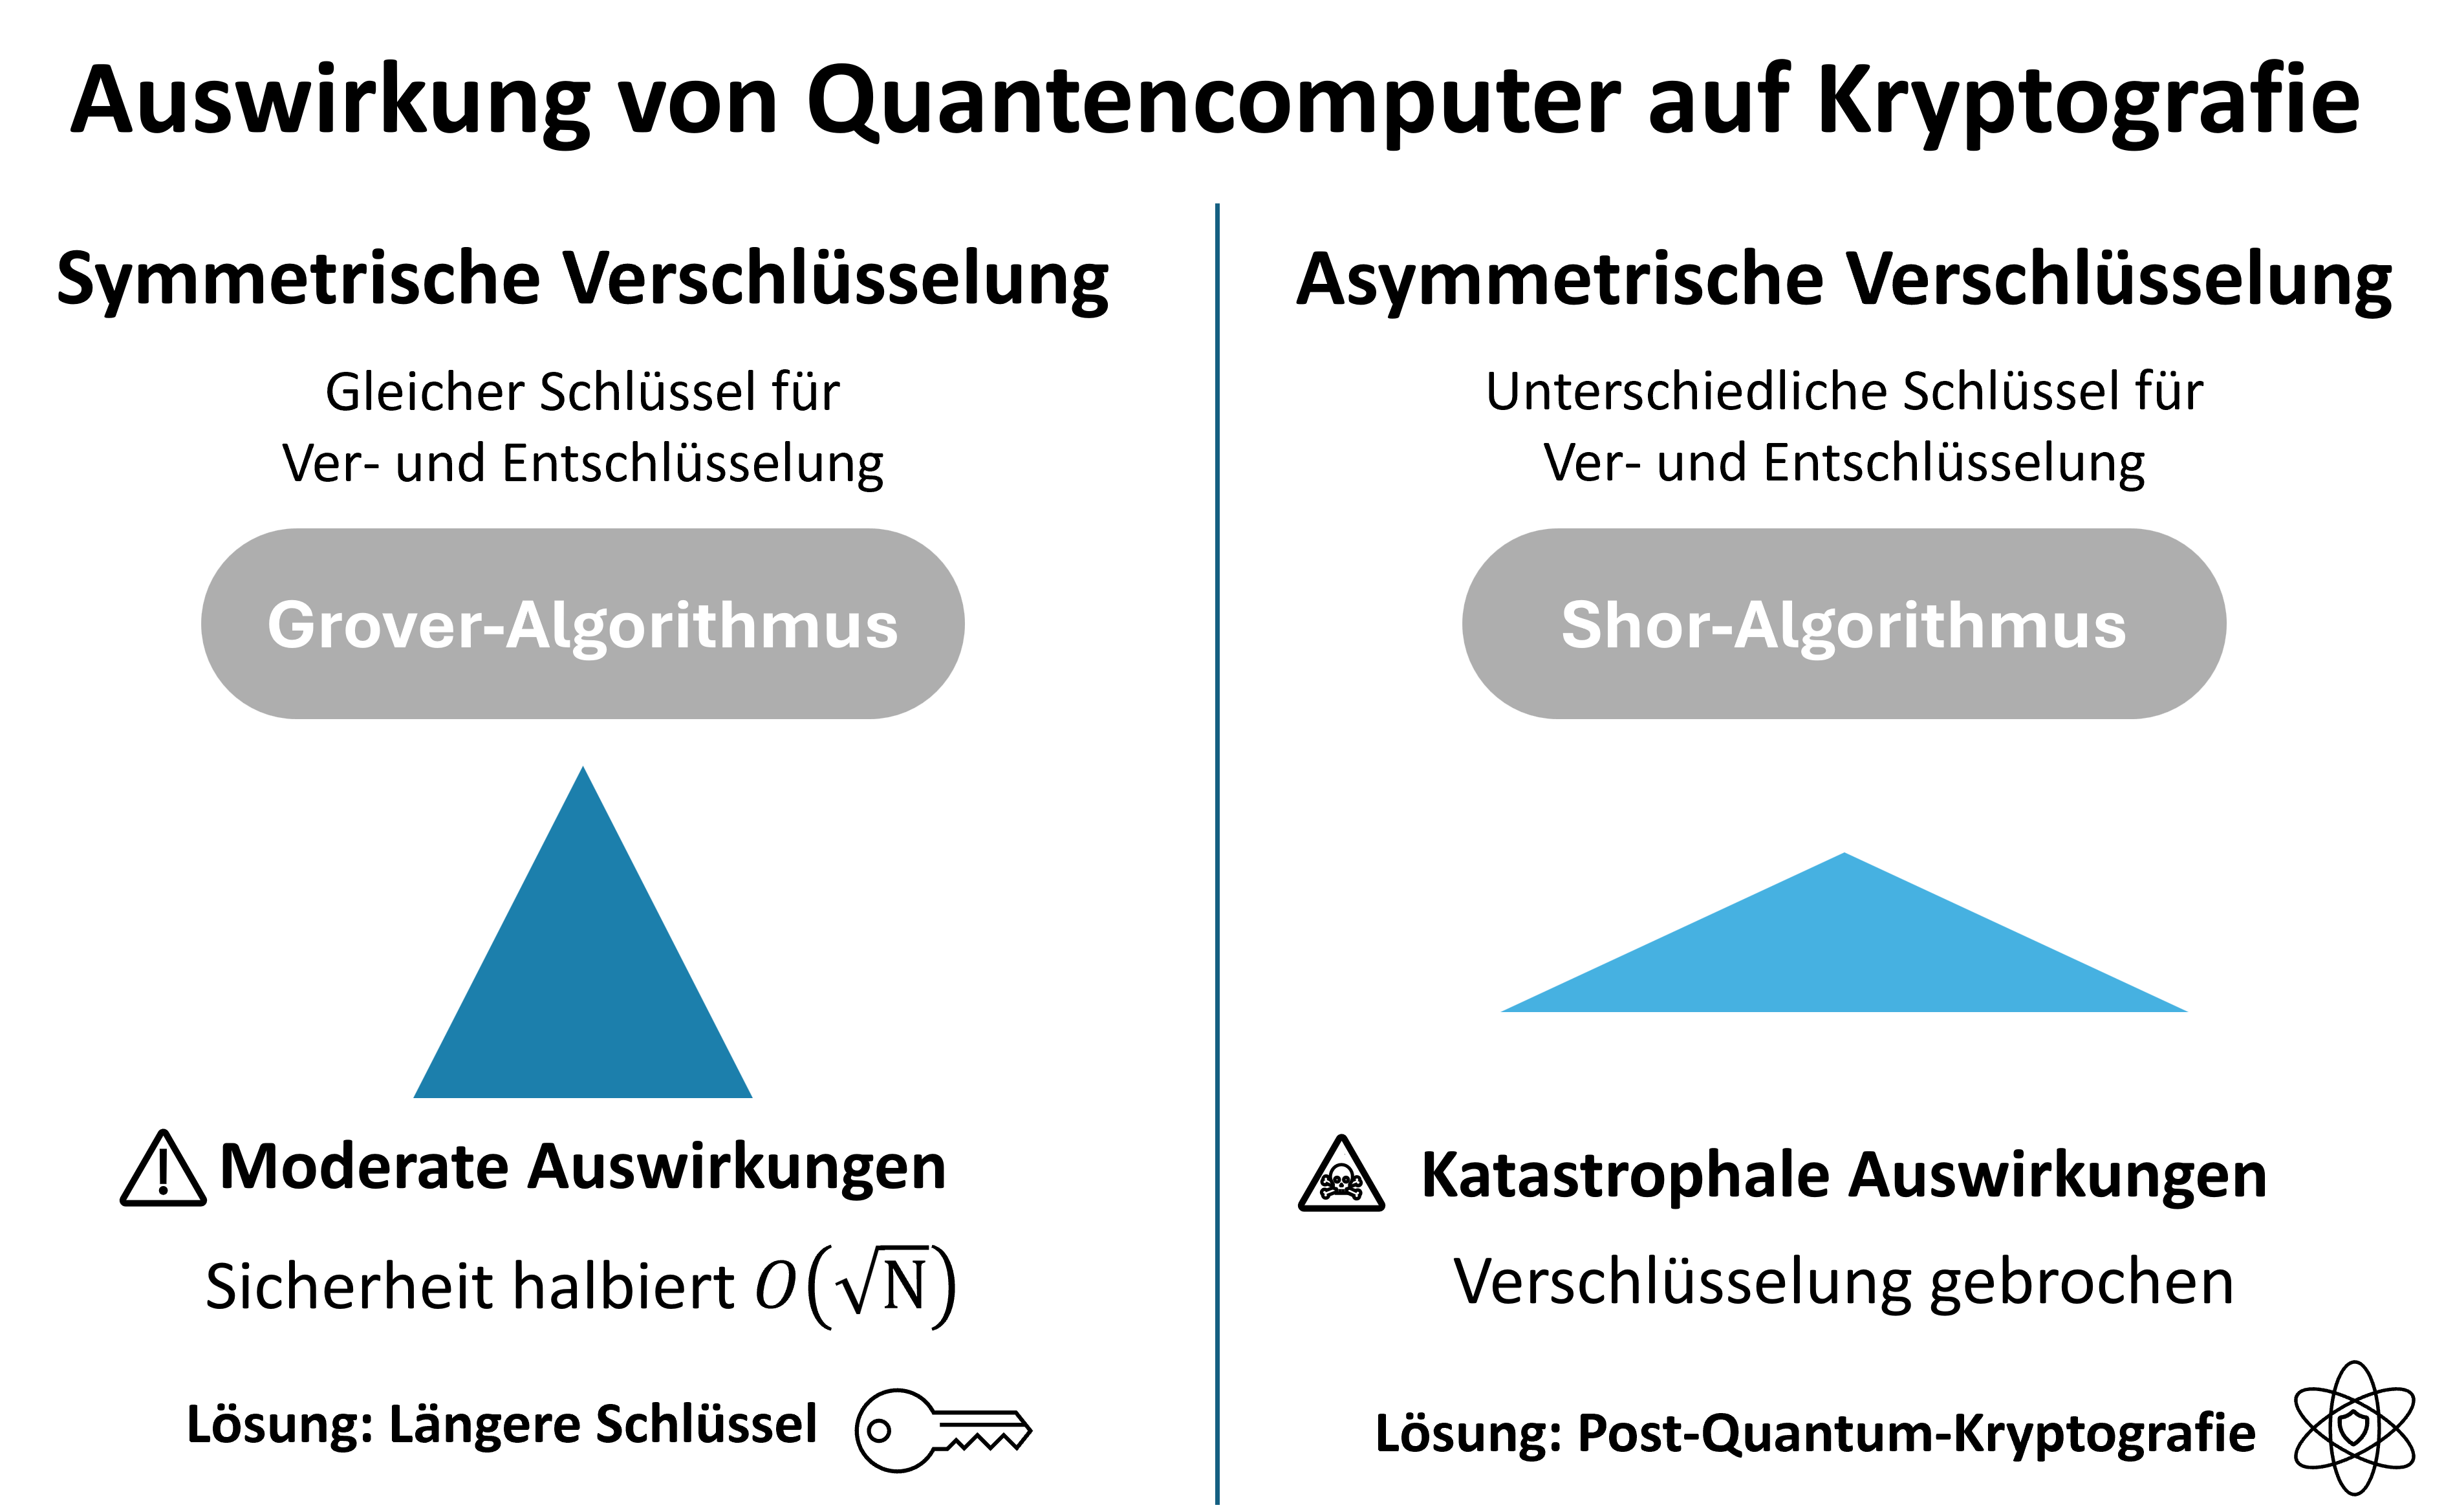
\includegraphics[width=1\linewidth]{images/Auswirkungen_Kryptografie.png}
    \caption{Sicherheitsbeurteilung verschiedener Verschlüsselungsverfahren. (Quelle: \cite{qday2030} - teilweise modifiziert).}
    \label{fig:encryption_security_level}
\end{figure}

\subsection{Grenzen der Sicherheit}
Moderne Informationssysteme sind heute stark von einer funktionierenden Verschlüsselung abhängig.
Es fällt nicht nur der Finanzsektor darunter, sondern die gesamte digitale Infrastruktur weltweit, das heisst auch staatliche
Verwaltungen, das Gesundheitswesen, industrielle Unternehmen sowie private Kommunikation \cite{menezes1996handbook}.
Gemäss Christian Weber setzen Anwendungen wie Online-Banking, E-Mail-Dienste, Cloud-Speicher oder auch die elektronische Identität (E-ID) auf sichere Verschlüsselung
ihrer Daten, um langfristig zuverlässig sein zu können.
Ein Versagen von genau diesen derzeit sicheren Verschlüsselungsverfahren würde somit nicht nur technische Probleme
verursachen, sondern auch wirtschaftliche und gesellschaftliche Konsequenzen nach sich ziehen \hyperlink{dependency_cryptography}{(siehe Interview im Anhang)}.
\\
Die heutige Sicherheit der Verschlüsselungsverfahren basiert primär auf der Annahme einer begrenzten Rechenleistung der klassischen Computer.
Asymmetrische Verfahren wie zum Beispiel RSA gelten als sicher, solange
keine praktikable Möglichkeit besteht, die zugrunde liegenden
mathematischen Probleme effizient zu lösen \cite{menezes1996handbook}.
Quantencomputer würden genau diese grundlegende Ausgangslage verändern,
da der Shor-Algorithmus die Faktorisierung grosser Zahlen in
realistischer Zeit ermöglichen kann \cite{mandrysch2016}.
Christian Weber bestätigt, die besten heutigen Verschlüsselungsverfahren wären nicht mehr sicher \hyperlink{dependency_cryptography}{(siehe Interview im Anhang)}.

\subsection{Harvest now, decrypt later}
Gemäss Christian Weber liegt ein zentrales Problem in der langfristigen Datensicherheit.
Daten, die heute verschlüsselt gespeichert werden, können zu einem späteren Zeitpunkt, bei Marktreife eines Quantencomputers, entschlüsselt werden.
Dies wird \emph{Harvest now, decrypt later}-Angriff (heute sammeln, später entschlüsseln) genannt \hyperlink{longterm_security}{(siehe Interview im Anhang)}.
\\
Besonders kritische Daten wie staatliche Geheimnisse, Gesundheitsdaten oder auch Finanzdaten sind davon betroffen.
Auch wenn die Daten momentan als sicher gelten, können diese zu einem
späteren Zeitpunkt entschlüsselt und kompromittiert werden \cite{mandrysch2016}.
\\
Trotz der bekannten Risiken, die durch die Entwicklung höherer
Rechenleistung durch Quantencomputer entstehen, so Christian Weber, werden momentan nur
wenige flächendeckende Massnahmen zur Entwicklung quantensicherer
Verfahren getroffen.
Viele Firmen und Institute sind sich der Problematik nicht bewusst oder
schätzen die Risiken zu gering ein (siehe Interview im Anhang).

\subsection{Gesamtbewertung}
Die aktuelle Sicherheitslage ist stark von der Annahme eines
stagnierenden Fortschritts in der Entwicklung der Quantencomputer
abhängig \cite{mandrysch2016}.
Sollte gemäss diese Annahme nicht eintreffen, wären die heutigen
Verschlüsselungsverfahren in ihrer Sicherheit stark gefährdet.
Zusammenfassend lässt sich sagen, dass die heutige Sicherheitslage als
funktional gilt, allerdings nicht zukunftssicher ist \hyperlink{overall_security}{(siehe Interview mit Christian Weber im Anhang).}
\pagebreak
\section{Zukunftsaussichten}
Angesichts der drohenden Gefahr durch Quantencomputer arbeiten Forschungseinrichtungen und Standardisierungsgremien weltweit an der Entwicklung quantensicherer Verschlüsselungsverfahren.
Das NIST hat bereits erste Standards für Post-Quanten-Kryptografie (PQC) Verfahren erarbeitet und im Jahr 2024 veröffentlicht \cite{nistpqc}.
PQC-Algorithmen sind so konzipiert, dass sie auf klassischen Computern laufen, aber gleichzeitig gegen Angriffe von Quantencomputern resistent sind \cite{srfEinsteinQuantencomputer}.
\\
Gemäss Christian Weber stellt die Umstellung auf PQC jedoch eine enorme Herausforderung dar.
Bestehende Systeme, Protokolle und Infrastrukturen müssen grundlegend überarbeitet werden, was erhebliche Investitionen erfordert.
Zudem fehlt es derzeit an koordinierten Umsetzungsplänen auf staatlicher und internationaler Ebene, was eine flächendeckende Migration erschwert \hyperlink{pqc_migration}{(siehe Interview im Anhang)}.
\\
Ein weiteres Problem ist die begrenzte Rechenleistung und Speicherkapazität bestehender Systeme.
PQC-Algorithmen benötigen oft grössere Schlüssel und mehr Rechenressourcen als herkömmliche Verfahren, was insbesondere bei älteren oder eingebetteten Systemen zu Kompatibilitätsproblemen führen kann \cite{fraunhoferPQC}.
%https://www.mhp.com/de/insights/blog/post/post-quantum-kryptographie
\\
Gemäss Christian Weber ist trotz dieser Herausforderungen die frühzeitige Vorbereitung auf die Post-Quanten-Ära unerlässlich.
Experten empfehlen, bereits heute mit der Planung und schrittweisen Implementierung quantensicherer Verfahren zu beginnen, um für den Zeitpunkt gewappnet zu sein, an dem leistungsfähige Quantencomputer verfügbar werden \hyperlink{pqc_migration}{(siehe Interview im Anhang)}.
\\
Grundsätzlich zielt Verschlüsselung nicht auf ewige Sicherheit ab, sondern nur darauf, 
Daten so lange zu schützen, bis sie ihren Wert verlieren wie z.B. Patente deren Schutz nach einigen Jahren abläuft \hyperlink{pqc_security}{(siehe Interview mit Christian Weber im Anhang)}.

